\documentclass [a4paper,11pt]{article}
\usepackage{amssymb}
\usepackage{amsthm}
\usepackage[intlimits]{amsmath}
\usepackage[polish]{babel}
\usepackage[utf8]{inputenc}
\usepackage[T1]{fontenc}
\frenchspacing
\usepackage{indentfirst}
\usepackage{graphicx}
\usepackage{subfig}
\usepackage{mathptmx}
\usepackage{geometry}
\usepackage{wrapfig}
\sloppy

\begin{document}
\newgeometry{tmargin=2cm, bmargin=2cm, lmargin=2cm, rmargin=2cm}

%----------- tabela nagłówkowa---------------------- %
\begin{table}[]
\centering
\begin{tabular}{lllllll}
\cline{1-6}
\multicolumn{1}{|c|}{\begin{tabular}[c]{@{}c@{}}EAiIB\\ Informatyka\end{tabular}}              & \multicolumn{2}{l|}{\begin{tabular}[c]{@{}l@{}}Autor 1\\ Autor 2\end{tabular}}                                                                                                & \multicolumn{1}{c|}{\begin{tabular}[c]{@{}c@{}}Rok\\ II\end{tabular}}          & \multicolumn{1}{c|}{\begin{tabular}[c]{@{}c@{}}Grupa\\ V\end{tabular}}            & \multicolumn{1}{c|}{\begin{tabular}[c]{@{}c@{}}Zespół\\ II\end{tabular}}      &  \\ \cline{1-6}
\multicolumn{1}{|c|}{\begin{tabular}[c]{@{}c@{}}Pracownia\\ FIZYCZNA\\ WFiIS AGH\end{tabular}} & \multicolumn{4}{l|}{\begin{tabular}[c]{@{}l@{}}Temat:\\ \textbf{Opracowanie danych pomiarowych} \end{tabular}}                                                                                                                                                                                                                                            & \multicolumn{1}{l|}{\begin{tabular}[c]{@{}l@{}}nr ćwiczenia:\\ 0\end{tabular}} &  \\ \cline{1-6}
\multicolumn{1}{|l|}{\begin{tabular}[c]{@{}c@{}}Data wykonania:\\ 7.10.2015\end{tabular}}      & \multicolumn{1}{c|}{\begin{tabular}[c]{@{}c@{}}Data oddania:\\ 14.10.2015\end{tabular}} & \multicolumn{1}{l|}{\begin{tabular}[c]{@{}l@{}}Zwrot do poprawki:\\ \phantom{data poprawki}\end{tabular}} & \multicolumn{1}{l|}{\begin{tabular}[c]{@{}l@{}}Data oddania:\\  \phantom{data oddania}\end{tabular}} & \multicolumn{1}{l|}{\begin{tabular}[c]{@{}l@{}}Data zaliczenia:\\  \phantom{data zaliczenia}\end{tabular}} & \multicolumn{1}{l|}{\begin{tabular}[c]{@{}l@{}}OCENA:\\ \phantom{ocena}\end{tabular}}       &  \\ \cline{1-6}
                                                                                               &                                                                                         &                                                                                     &                                                                                &                                                                                   &                                                                               & 
\end{tabular}
\end{table}

\section{Wstęp}
Wahadłem matematycznym nazywamy ciało masie $m$ i o niezmiernie małej objętości (czyli punkt materialny), zawieszone na nieważkiej i nierozciągliwej nici o długości $l$ . W praktyce takim wahadłem jest ciało, którego wymiary liniowe są znacznie mniejsze od długości nici.
Jeśli wahadło wychylimy o niewielki kąt $\alpha$ to jego okres można wyrazić wzorem:
$$ T= 2 \pi \sqrt{\frac{l}{g}} $$

Przekształcając ten wzór możemy wyznaczyć wartość przyspieszenia ziemskiego:
$$ g= \frac{4 \pi^2 l}{T^2} $$


\section{Układ pomiarowy}
Badane wahadło stanowi mosiężny obciążnik zawieszony na cienkiej lince. Linka jest podwieszona na
wolnostojącym statywie. Pomiary były dokonywane za pomocą stopera o dokładności 0,01 s. Do niepewności pomiaru stopera należy dodać czas reakcji osoby wykonującej pomiary, który został ustalony na $0,1 s$. Długość wahadła wyznaczono mierząc
długość linki miarką o dokładności 1 mm. Dokładność wyznaczenia długości wahadła jest jednak zdecydowanie mniejsza (konieczność oszacowania odległości mocowania linki do środka kulki,punkt zawieszenia linki) i została określona na 5 mm. Długość linki może być regulowana.

\begin{figure}[h!]
\centering
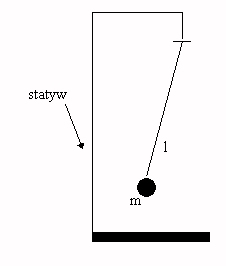
\includegraphics[width=0.3\linewidth]{./wahadlo}
\caption{Schemat wahadła matematycznego}
\label{fig:wahadlo}
\end{figure}

\section{Wykonanie ćwiczenia}
 \subsection{Wyznaczenie przyspieszenia ziemskiego:}
\begin{enumerate}
\item Zmierzenie długości linki, poczynając od środka obciążnika(nie jest możliwe dokładne wyznaczenie środka obciążnika, co powoduje błędy pomiaru)
\item Wychylenie wahadła o niewielki kąt z położenia równowagi i puszczenie
\item Odczekanie aż wahania się ustabilizują
\item Zmierzenie przy pomocy stopera 10 pełnych okresów wahadła
\end{enumerate}

 \subsection{Badanie zależności okresu drgań od długości wahadła}
Pomiary są wykonywane podobnie jak w poprzedniej części doświadczenia. Zmierzono czas trwania 10 pełnych okresów wahadła dla 7 różnych długości linki. 

\section{Wyniki i ich opracowanie}
\subsection{Wyznaczanie wartości przyspieszenia ziemskiego}


\begin{figure}[h!]
\centering
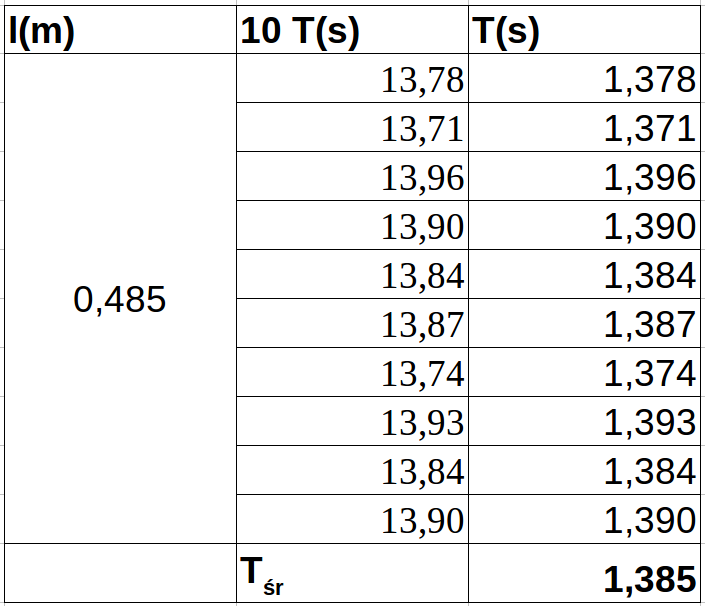
\includegraphics[width=0.5\textwidth]{./tabelka_10_pomiarow}
\caption{Wyniki pomiarów 10 okresów wahadła}
\label{fig:tabelka_10_pomiarow}

\end{figure}


 Najbardziej prawdopodobną wartością okresu jest
wartość średnia: 
$$ T_{\text{śr}}  = \frac{1}{n} \sum_{i=1}^{n} T_i $$
Wartość przyspieszenia ziemskiego:
$$g= \frac{4 \pi ^2 l}{ T_{\text{śr}}^2} = \frac{4 \cdot 3,141^2 \cdot 0,485} {1,385^2} \approx 9,986 \left[ \frac{m}{s^2} \right] $$


\newpage


\subsection{Badanie zależności okresu drgań od długości wahadła}
\begin{figure}[h!]
\centering
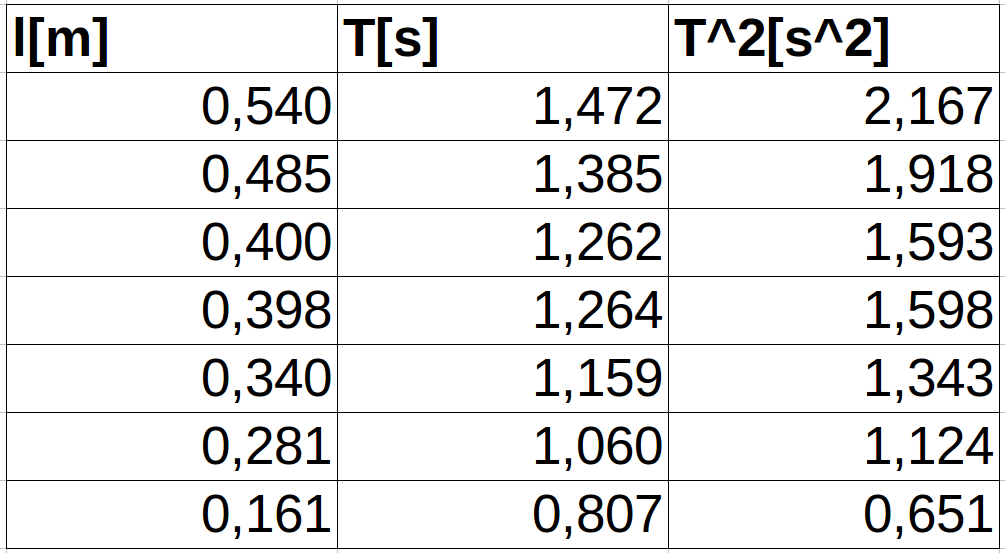
\includegraphics[width=0.7\linewidth]{./tableka_pom}
\caption{Tabela pomarów dla badania zależnośći okresu drgań od długości wahadła}
\label{fig:tableka_pom}
\end{figure}

 Wykres $T(l)$ jest wykresem typu $y= \sqrt{x}$, który jest trudny w analizie

\begin{figure}[h!]
\centering
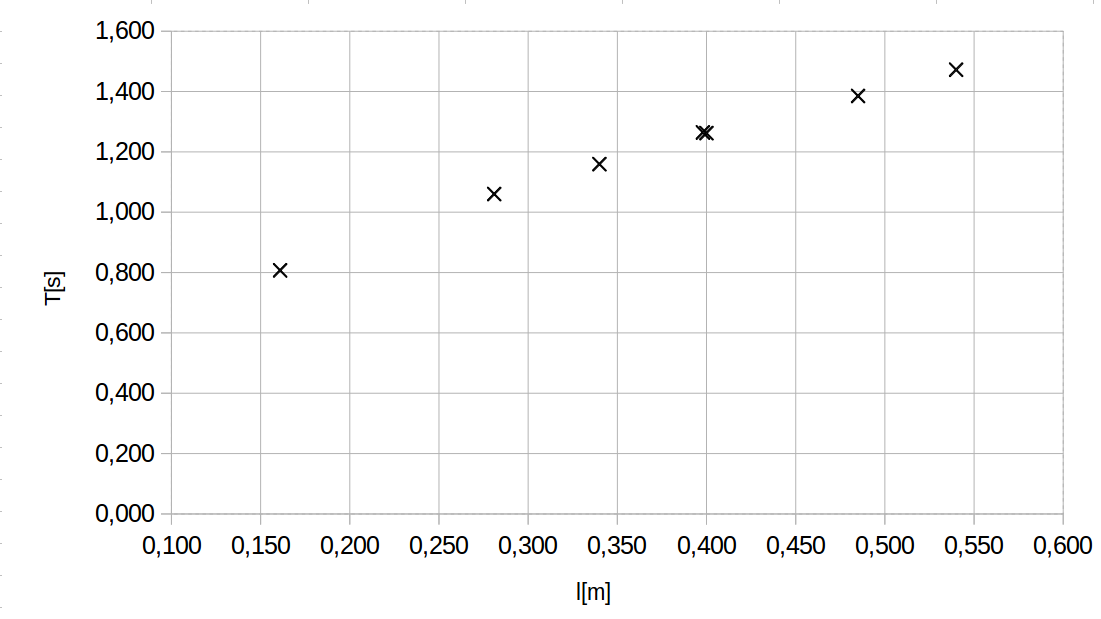
\includegraphics[width=0.7\linewidth]{./wykres_l(T)}
\caption{Wykres $T(l)$}
\label{fig:wykresl(T)}
\end{figure}

Podnosząc wzór na okres wahadła matematycznego obustronnie do kwadratu otrzymamy następującą zależność:
$$ T^2 = \frac{4 \pi^2}{g} l $$ 
Wykres tej zależności przedstawionej na Rysunku~\ref{fig:wykresT^2(l)}  jest liniowy.
Poniżej przedstawiony jest wykres zależności $T^2(l)$ od długości wahadła wraz z linią regresji uzyskany przy pomocy programu Excel
  
\begin{figure}[h!]
\centering
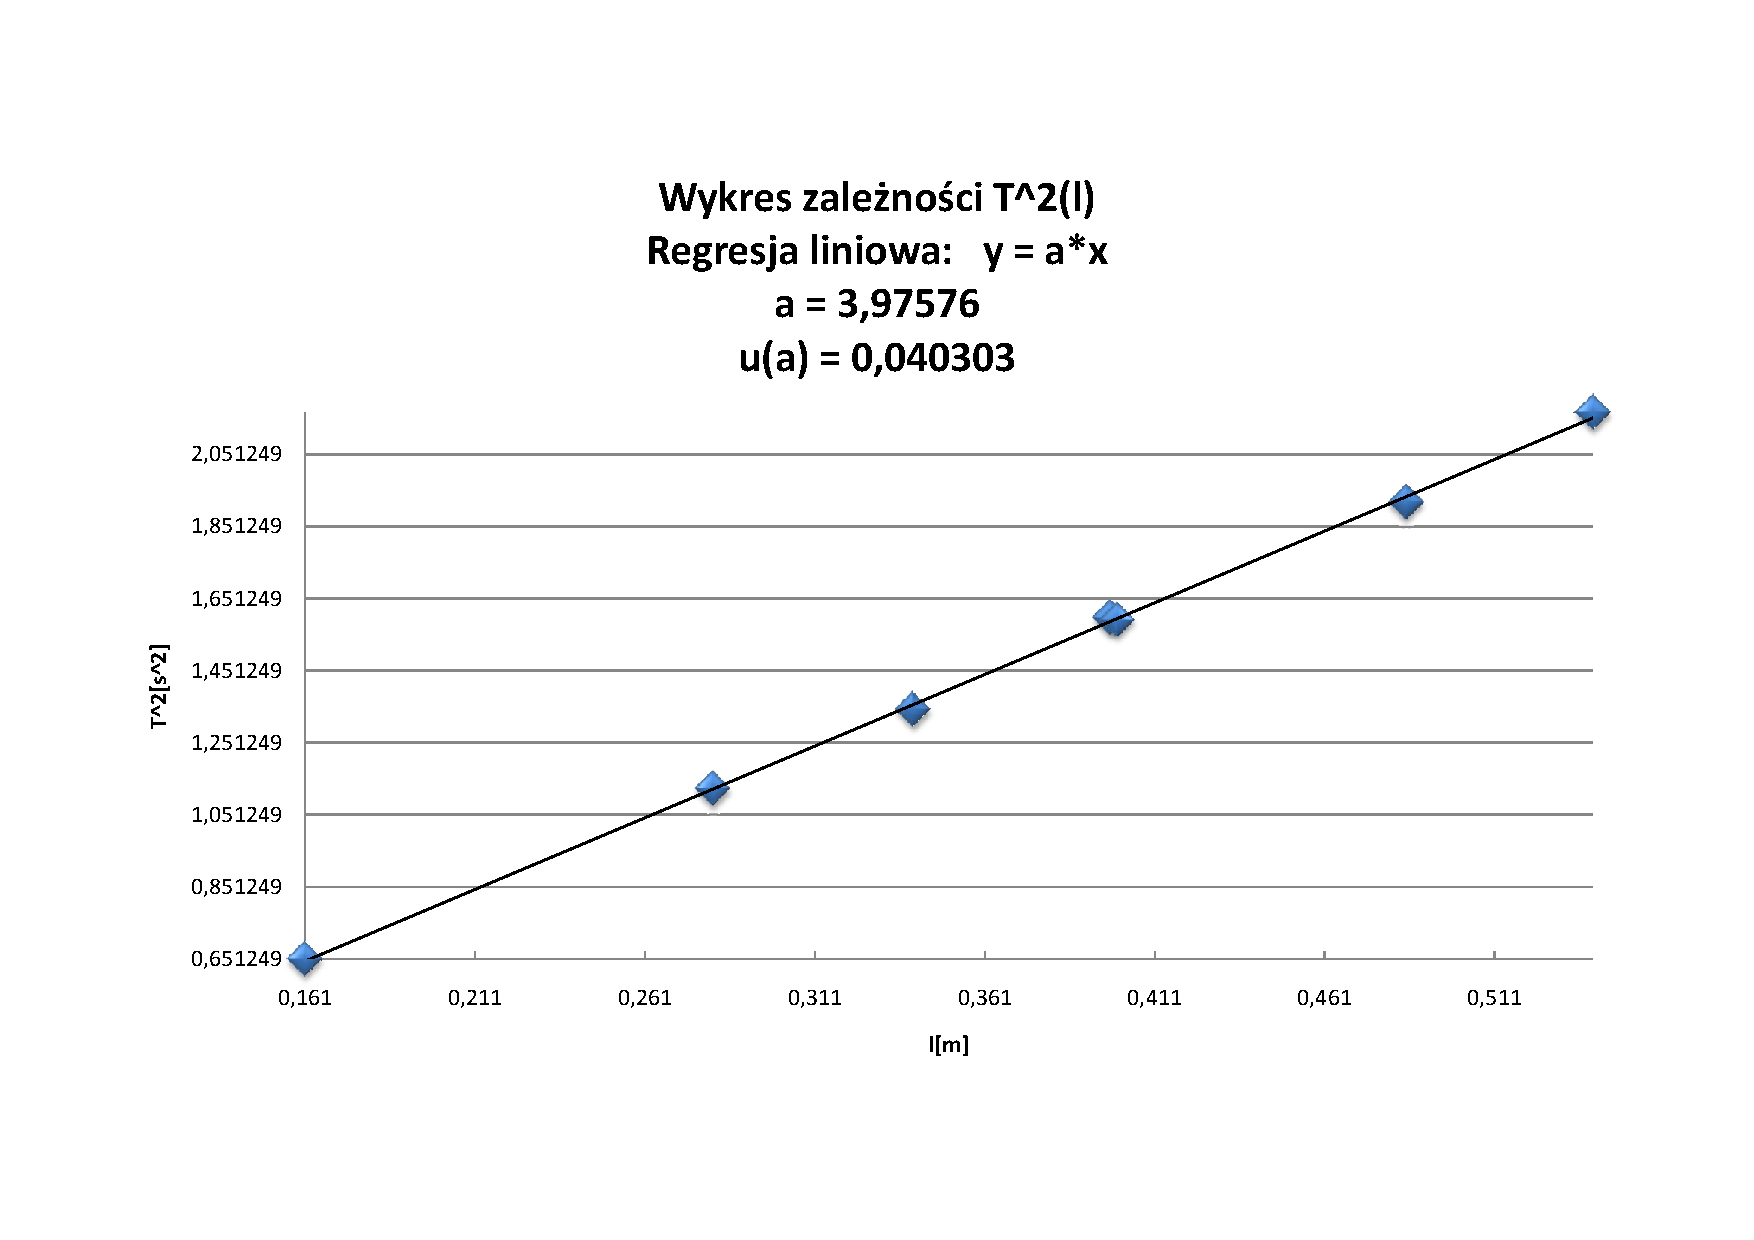
\includegraphics[width=0.7\linewidth]{./wykresT^2(l)}
\caption{Wykres $T^2(l)$}
\label{fig:wykresT^2(l)}
\end{figure}


Znając współczynnik $a$ nachylenia wykresu możemy wyznaczyć przyspieszenie ziemskie $g$:
$$ T^2 = \frac{4 \pi^2}{g} l $$
$$ a =   \frac{4 \pi^2}{g} \Longrightarrow g= \frac{4 \pi^2}{a}  \approx 9,930 \left[ \frac{m}{s^2}\right]  $$  
\section{Szacowanie niepewności pomiarowych}
\subsection{Wyznaczanie wartości przyspieszenia ziemskiego}
\subsubsection{Niepewność pomiaru okresu}
Jako, że posiadamy serię pomiarów okresu wahadła dla tej samej długości, jego niepewność obliczamy metodą typu A, czyli jako estymator odchylenia standardowego wielkości średniej:
$$ u(T)  = \sqrt{\frac{\sum_{i=1}^{n} \left(T_i - T_{\text{śr}}\right)^2}{n(n-1)}} \approx 0,0026 [s] $$
\subsubsection{Niepewność pomiaru długości wahadła}
Niepewność pomiaru długości jest szacowana na podstawie dokładności pomiaru:
$$u(l) = \frac{\Delta l}{\sqrt{3}} = \frac{0,005}{\sqrt{3}} \approx 0,0029 [m] $$
\subsubsection{Niepewność złożona pomiaru przyspieszenia ziemskiego}
Jako, że przyspieszenie ziemskie jest wyznaczane pośrednio, stosuję prawo przenoszenia niepewności:
$$u_c(g) = \sqrt{\left(  \frac{\delta g}{\delta T} \right)^2 u(T)^2 + \left( \frac{\delta g}{\delta l} \right)^2 u(l)^2  } = \sqrt{\frac{64 \pi^4 l^2}{T^6} U(T)^2 + \frac{16 \pi^4}{T^4} u(l)^2}\approx 0,070 \left[ \frac{m}{s^2} \right] $$

Aby porównać wyznaczoną wartość z wartością tablicową obliczamy niepewność rozszerzoną:
$$U_c(g) = k \cdot u_c(g) = 2 \cdot 0,070 = 0,140 \left[ \frac{m}{s^2} \right] $$
 
Tak więc wyznaczone przyspieszenie ziemskie ma wartość:
$$g = (9,986 \pm 0,140)\left[ \frac{m}{s^2} \right] $$  
Wartość tablicowa przyspieszenia ziemskiego wynosi $g= 9,811 \left[ \frac{m}{s^2} \right] $ i  nie mieści się w wyznaczonym przez nas przedziale.

\subsection{Badanie zależności okresu drgań od długości wahadła}
Ponownie stosujemy prawo przenoszenia niepewności. Tym razem mamy do czynienia z funkcją jednej zmiennej:  $g= \frac{4 \pi^2}{a}$
$$ u(g) = \frac{\delta g}{\delta a} u(a) =  - 4 \pi^2 a^{-2} \cdot u(a)$$
$$ |u(g)| =  4 \pi^2 a^{-2} \cdot u(a) \approx 0,101  \left[ \frac{m}{s^2}\right] $$
$$U_c(g) = k \cdot u_c(g) \approx 2 \cdot 0,101 = 0,202 \left[ \frac{m}{s^2} \right] $$
Tak więc przyspieszenie ziemskie wyznaczone na podstawie wykresu zależności $T^2(l)$ ma wartość:
$$g = (9,930 \pm 0,202)\left[ \frac{m}{s^2} \right] $$

\section{Podsumowanie pomiarów}
\begin{tabular}{|c|c|c|c|}
\hline Opis wielkości & Wynik $\left[ \frac{m}{s^2} \right]$ & u(g) $\left[ \frac{m}{s^2} \right]$ & $U_c(g)$ $\left[ \frac{m}{s^2} \right]$ \\
\hline $g$ za pomocą 10 pomiarów przy tej samej dł wahadła  & 9,986 & 0,070  & 0,140  \\ 
\hline $g$ za pomocą wykresu $T^2(l)$ & 9,930  & 0,101  & 0,202  \\ 
\hline Wartość tablicowa $g$ & 9,811  & -  & -  \\ 
\hline 
\end{tabular} 



\section{Wnioski}
\begin{itemize}
\item Wahadło matematyczne jest dosyć dokładnym i prostym do wykonania sposobem wyznaczenia przyspieszenia ziemskiego, ponieważ uzyskane niepewności są niewielkie
\item Zakres uzyskanej wartości przyspieszenia ziemskiego wraz z niepewnością uzyskanych za pomocą badania wykresu $T^2(l)$ zawiera w sobie wartość tabelaryczną przyspieszenia ziemskiego, a w przypadku drugiej metody zakresy niepewności mijają wartość tabelaryczną o bardzo małą wartość. Świadczy to o poprawności pomiarów
\item Powodem uzyskania wyniku odchylonego od wartości rzeczywistej może być fakt, że wahadło mogło poruszać się w więcej niż jednej płaszczyźnie

 
\end{itemize}

\end{document}